\documentclass[11pt]{article}
\usepackage{graphicx}
\graphicspath{ {images/} }

\begin{document}

\title{%
 Agile TweetViz from team Geek!O\\
\large Project Report}
\author{Harsha Kadekar\\
  Yash Chopra\\
  Gowtham Nayak\\
  Anoop Jatavallabha\\
  Seema Suresh}
\date{\today}
\maketitle
\newpage
\tableofcontents
\newpage
\listoffigures
\newpage


\section{Introduction}
The popularity of social media has made twitter an important platform for information transfer, news reporting and public opinion. Despite the significant potential for measuring public opinion, finding the perspective for any topic by sorting through massive number of tweets is an arduous task. In this project , we try to establish the relationship between different aspects of tweets and further visualize them for easy interpretation. This program also has the capacity to download, analyze and visualize the tweets for any mentioned topic present or past.
 
The tweets are fetched based on user given topics, where topics can be anything from a word to few sentences. This process is achieved by using two	 separate libraries in Python: NTLK library (Natural Language Toolkit) and Tweepy library. For analyzing tweets, a smalltalk based platform “Moose/Pharo” is used where a metamodel is defined which in turn will feed data for visualization. Finally, visualization is achieved using Roassal library in Pharo.
 
We have demonstrated assorted visualization, trying to utilize the maximum power of Roassal library, while establishing relationship between different aspects of tweet and its user. Further, our paper is divided as follows: 2) Understanding hashtag relation 4-5) Requirements 6) Architecture 11-12) Outcomes and Future work.

\section{Understanding hashtag relations of software engineering tweets}
Twitter is a platform, where individuals can express their views by using sentences having 140 characters or less. These tweets can further be liked or retweeted by other followers, thus increasing the area of viewership among the users of Twitter. Another important characteristics of Twitter is the association of tweets with a certain topic by using "hashtags". A hashtag is created by placing a "\#" in-front of a word. By doing so, a tweet can be tagged to a certain topic. A tweet can have a single or multiple hashtags thus representing either one or multiple topics simultaneously. For example, to express a security concern in Java, a tweet can be mentioned as \textit{"A prog example of trojan using Java. Be aware of threat! \textbf{\textit{\#java \#security}}"} or to announce a job posting a tweet can be mentioned as \textit{"Experienced software engineers needed for front end development. DM me details. \textbf{\textit{\#javascript \#UIdesign \#jobs}}"}. By mentioning more than one hastag in a tweet, a user is trying to establish the relationship between two different topics. Therefore, in our second example, we can find same tweet by searching \#javascript and \#jobs. 

For this project,our first aim is to understand the relationship between the hashtags present in tweets related to Software Engineering . Secondly, we have utilized this relationship to categorize the tweets and tweet handlers into different groups. Finally, we have tried visualizing the analyzed tweets and their relationship so as, this information can be conveyed in a much compact and simpler manner. This analysis will help us to determine the popularity of an user in a particular field of interest. For example, user is tweeting on the topics related to \#Java, \#Security, \#Job, \#Issue, and \#JDK. Among these topics, \#Security is the most popular hashtag. This condition can be determined based on the counts of retweets and number of likes on a tweet. Our aim is to clearly understand user area of expertise. In this case, it is Java Security even though user is tweeting about issues, job and jdk.

\section{Development Process}
For this project we have used Agile process with Scrum methodology. The main reason to choose this process was for its ability to handle change effectively. Taiga and Google site were used for implementation of software process where as Git was used for change management. These topics have been further discussed in the following subheadings: Project Plan, Management Plan, Implementation, Verification and Validation.
\section{Requirements: Problem Statement and Specifications}
Our project description as mentioned in the SCORE website is 

"The popularity of social media has made Twitter a reliable platform for measuring social opinion. Unfortunately, giving a meaning to a massive number of tweets is challenging, despite the significant potential for measuring public opinion. This project is about creating an agile Tweet visualization engine. This engine should provide the ability to easily craft and tailor visualizations of a possibly large number of tweets. Visual patterns, emerging from the visualizations, will indicate facts. Visualizations should provide a way to easily navigate and crawl over tweets. Scope of the Project - Regarding the technical part of this project, it is (highly) suggested:
\begin{itemize}
\item to first define a meta-model for Tweets using the Moose platform;
\item to build the visualization engine on top of the Roassal visualization engine;
\item to carry out some tasks based on actual public opinions." \cite{SCOREwebsite}
\end{itemize}

We have gathered and refined our requirements by conducting Brain Storming sessions with the team and Online Meetings with our project sponsor. As sprints proceeded, our understanding of the new tool - Roassal in Pharo increased , which in turn helped to explore new possibilities for the product. 

From the problem statements, it was clear that we had two process requirements: 1) Meta-model was required to be created in MOOSE platform 2) Visualization were to be performed using Roassal. As both the platforms were new to us, the main task in our first sprint was to understand them. We went ahead and generated our first set of product related user stories. This involved user requirements like "As a user, I want to fetch tweets based on a given topic.", "As a user, I would like to give the input in a web page", "As a user, I would like to develop a meta model of the downloaded tweets", "As a user, I would like to develop a visualization of the meta-model". As the user stories were vague, we discussed this problem with our sponsor Dr Alexander Bergel, Dr. Kevin Gary and later conducted brainstorming sessions to create better user stories. We decided to place more emphasis on Meta-model creation and visualization, rather than user interface. 

Agile helped us to continuously add or change the requirements without hindering the product development. At the end of first sprint, requirements related to fetching of tweets were finalized while, still debating on meta-model and visualization. Requirements for Meta-model and Visualization were finalized at the end of sprint 2 and sprint 3 respectively. We discussed with the sponsor after the 4th sprint and the incorporated the changes to the existing requirements. Any unclear requirement acted as a placeholder for a conversation with the product owner to better understand the requirement. Software requirement Specification was updated throughout all the sprints.

\section{Architectural Design}
The three main modules of this project are: - 1) Tweet Fetch 2) Tweet Analysis 3) Tweet Visualization

\begin{figure}[h]
\centering
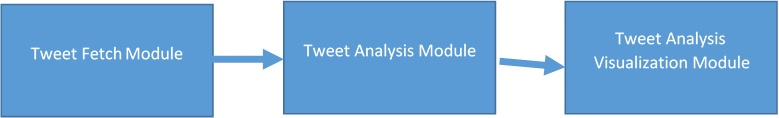
\includegraphics[width=\textwidth]{HighLevelDesign.jpg}
\caption{High Level Modules}
\end{figure}
\subsection{Tweet Fetch}
Tweet fetch Module is responsible for fetching tweets based on user input. This module can further be divided into three main parts: Processing user input, Fetching tweets and Storing tweets. A user input can be anything from a single word to a complete sentence , which is then parsed to generate hashtags. These hashtags are used to search and download the relevant tweets. Once the tweets are downloaded, they are stored in SQL tables and CSV file. Our next module, Tweet Analysis, directly takes CSV file as input. We chose MySQL over SQL Express, because of its ability to store large number of tweets.

DataStorageReader as outlined in figure 2, is a singleton class and is responsible for reading configuration file, interacting with TweetViz MySQL DB and interacting with CSV file through filereaderwriter component. Configuration file contains following parameters - 
\begin{enumerate}
\item SQL connection related parameters.
\item Type of tweets fetched - Most recent, Popular, Mixed.
\item Type of storage - CSV or SQL.
\item CSV file path.
\item Debug level.  
\end{enumerate}

\begin{figure}[h]
\centering
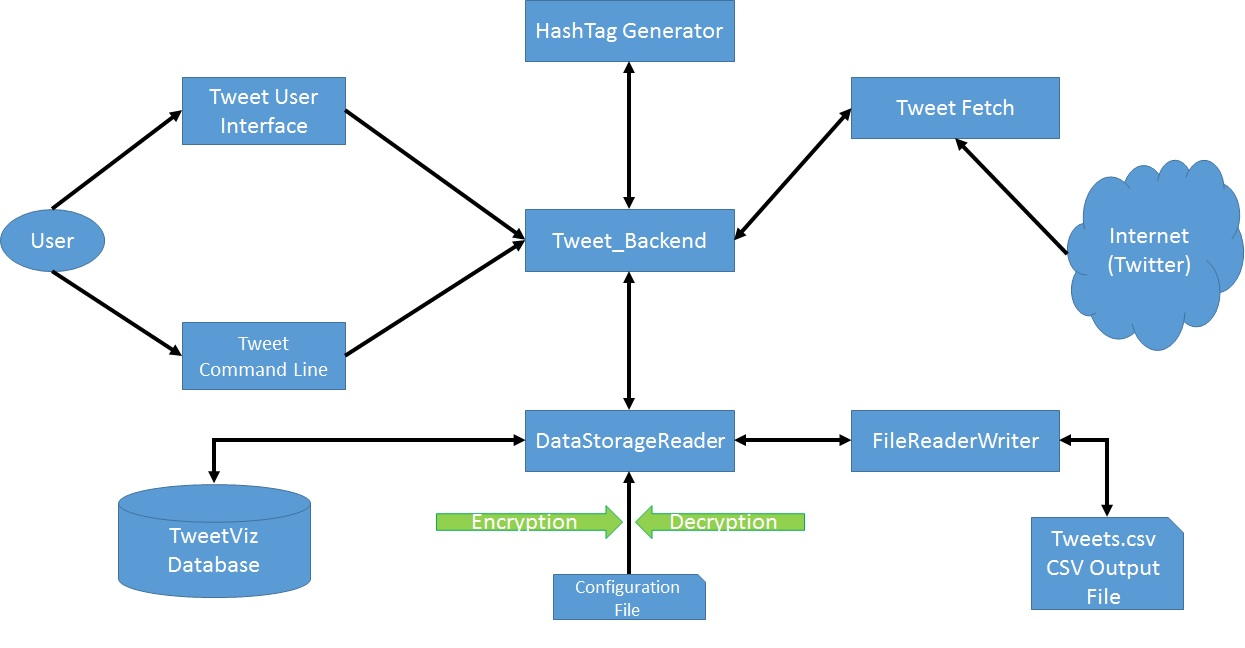
\includegraphics[width=\textwidth]{TweetFetch.jpg}
\caption{High Level Design of Tweet Fetch Module}
\end{figure}

For security reasons, Sql parameters are encrypted and stored in configuration file. HashtagGenerator is responsible for generating the hashtags from the given user input using natural language processing. TweetFetch component will get the tweets from Twitter based on the given hashtags. TweetBackend is responsible for the integration of all the different components.

\subsection{Tweet Analysis}
Two main responsibilities of this module are: Read the tweets and Generate the metamodel. CSVFileToTweetVizModel as outlined in figure 3, will use Neo-CSV package of MOOSE to read the CSV file and further generate the metamodel. Metamodel has inter-related objects representing Tweet, Tweet-User, HashTag and SearchCategory. 

\begin{figure}[h]
\centering
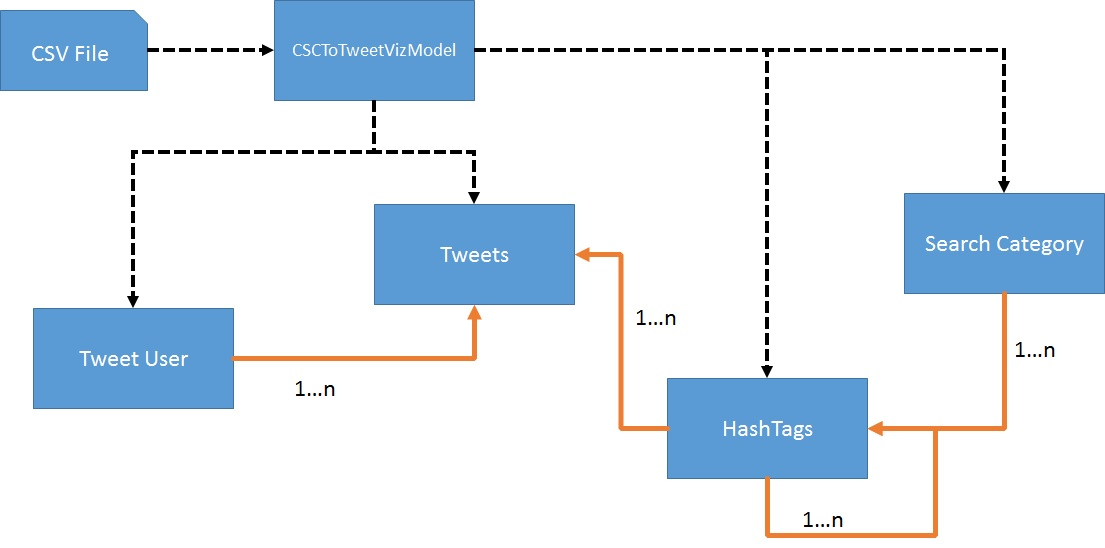
\includegraphics[width=\textwidth, height=5cm]{TweetAnalysis.jpg}
\caption{High Level Design of Tweet Analysis}
\end{figure}

\subsection{Tweet Visualization}
Multiple visualizations are generated representing the relationships between different objects of the metamodel. To achieve this, we have used RTView and Roassal class in Pharo/MOOSE.

\section{Project Plan}
Project development was divided into five iterations. First sprint was utilized for understanding of requirements and analysis of tools; next 3 sprints were dedicated for development of the major technical components of product; and last sprint was allocated for integration, testing and documentation. Major step stones of the project can be described as - 
\begin{enumerate}
\item Sprint 1 (21 SEP 2015-05 OCT 2015): - On second Saturday of the 2-week sprint, the following agendas were accomplished:
\begin{itemize}
\item Demonstrate different tools mentioned in requirements as learned by team members.
\item Participate in brainstorming session to further elaborate  the requirements of the project.  
\end{itemize}
\item Sprint 2 (05 OCT 2015-19 OCT 2015): - On second Saturday of the 2-week sprint, the following agendas were discussed/ demonstrated:
\begin{itemize}
\item Obtain user input in the form of a word or a sentence.
\item Parse the user sentence to build hashtags.
\item Fetch the tweets based on hashtags.
\item Store the fetched tweets.
\end{itemize}
After this sprint, the demo was presented in front of an external reviewer, Dr. Kevin Gary and the his inputs were used to make technical and procedural changes to our project.

\item Sprint 3 (19 OCT 2015-02 NOV 2015): - On second Saturday of the 2-week sprint, the following agendas were discussed/ demonstrated:
\begin{itemize}
\item Analyze the data to produce Tweet objects in Pharo.
\item Analyze the data to produce Hashtag objects in Pharo.
\item Analyze the data to produce User (Twitter handles) objects in Pharo.
\item Analyze the data to produce Search Category (Application user input) objects in Pharo.
\end{itemize}
The working model will demonstrate meta-model containing several objects. These objects will be further used in Roassal library for the visualization thus offering user the opportunity to review the topics of visualization.
\item Sprint 4 (02 NOV 2015-16 NOV 2015): - On second Saturday of the 2-week sprint, the following agendas were discussed/ demonstrated:
\begin{itemize}
\item Visualize Hashtag tree relationship.
\item Visualize Hashtag and Tweet words cloud relationship.
\item Visualize User, Tweet and hashtag organization chart relationship.
\item Visualize User and Tweet connection circle relationship.
\item Visualize tweet messages of different tweets.
\end{itemize}
The demo will present different visualization based on generated meta-model. There are several different types of Smart-arts and chats presented to demonstrate the wide range of visualization power of Roassal library in Pharo.
\item Sprint 5 (16 NOV 2015-23 NOV 2015) – On second Saturday of the 2-week sprint, the following agendas were discussed/ demonstrated:
\begin{itemize}
\item Integrate all the modules of the product.
\item Complete documentation related to product and project.
\item Full system run from user input to final visualization
\end{itemize}
The focus of this sprint was on the integration of separate modules and testing the code in parts and in full. The system needed to perform flawlessly.

\end{enumerate}

\section{Management Plan}
We followed Agile work environment with two weeks of sprint duration and conducted stand-up meetings on every alternate day. For every sprint meeting, the first half was dedicated to sprint review and second half of the meeting was reserved for sprint planning. Sprint review focused on the following points:
\begin{itemize}
\item Which tasks were left incomplete and the reasons behind them?
\item What worked well for us? What did not worked well for us? What actions can we take to improve our process?
\end{itemize}
In the sprint planning, following things were discussed:
\begin{itemize}
\item Objective of the new sprint.
\item Any new user stories or any change to the priority of the user stories in product backlog?
\item Which users stories needed to be moved from product backlog to sprint backlog?
\item Allocation of tasks and roles of different team members.
\end{itemize}

Three questions answered by each team member in the daily stand-up meeting were 1) What did I do? 2) What I will be doing till next meeting? 3) Is there any issue which team must know OR Is there any help needed from the team? 

Two tools helped us monitor the whole process - Taiga and Google Site. Taiga was used as our visual management board that helped us to keep record of the product backlogs(figure 4) and sprint backlogs (figure 3).

Once the user story has been moved from the product backlog to the sprint backlog, the state of the tasks of user stories can be monitored during that sprint as: New, In progress, Testing or Completed.

\begin{figure}[!ht]
\centering
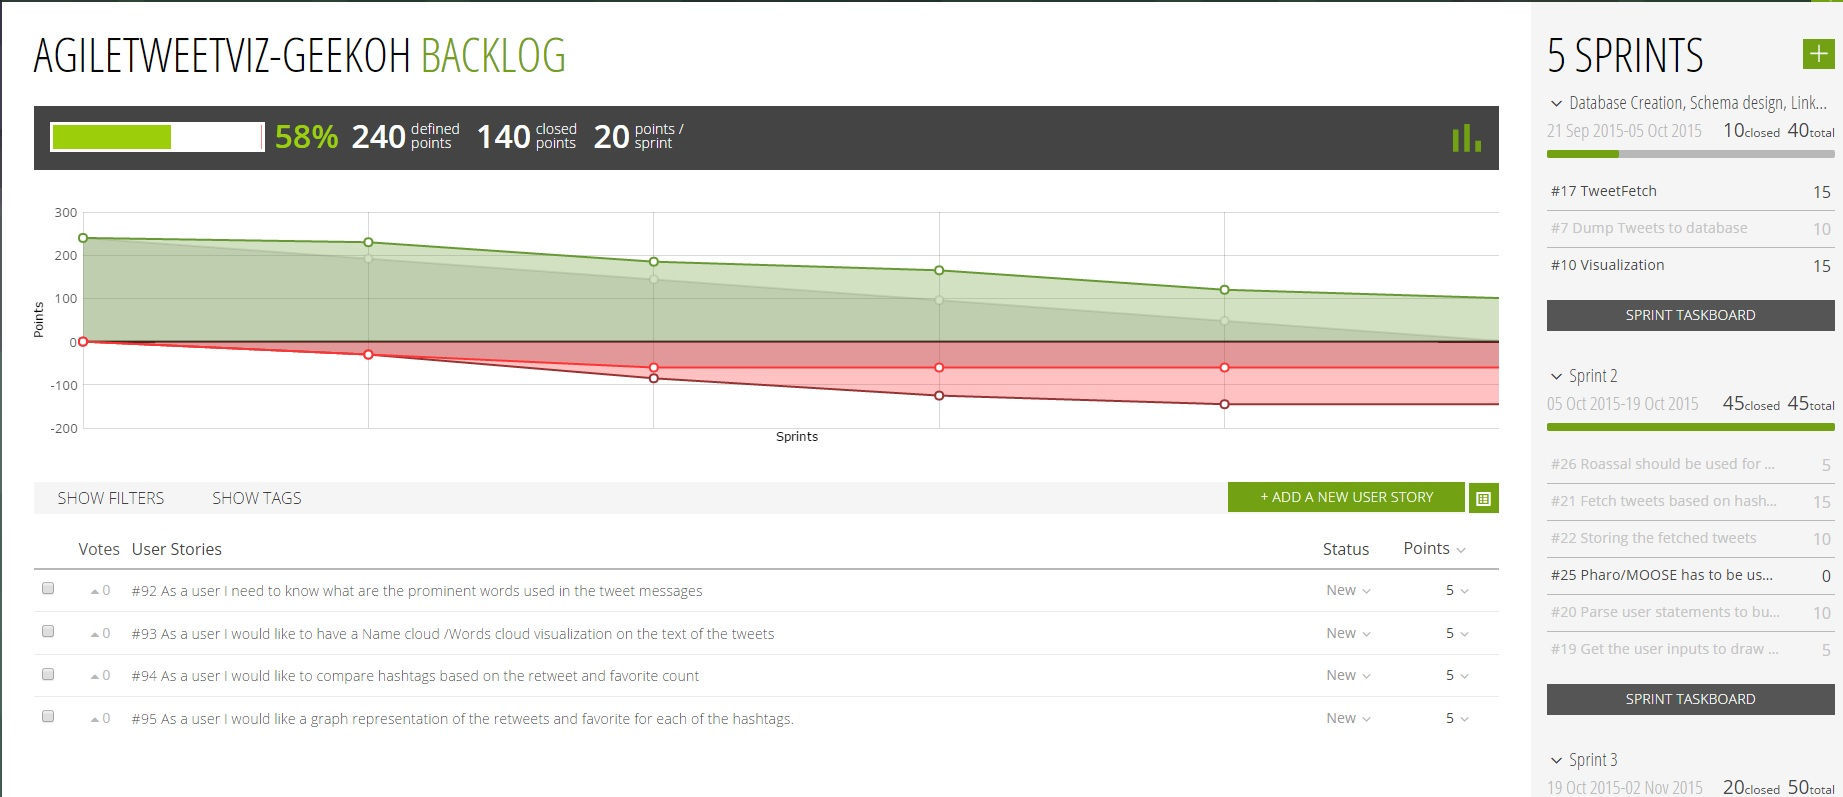
\includegraphics[width=6cm, height=6cm]{Backlog.jpg}
\caption{Product backlogs in Taiga}
\end{figure}

\begin{figure}[!ht]
\centering
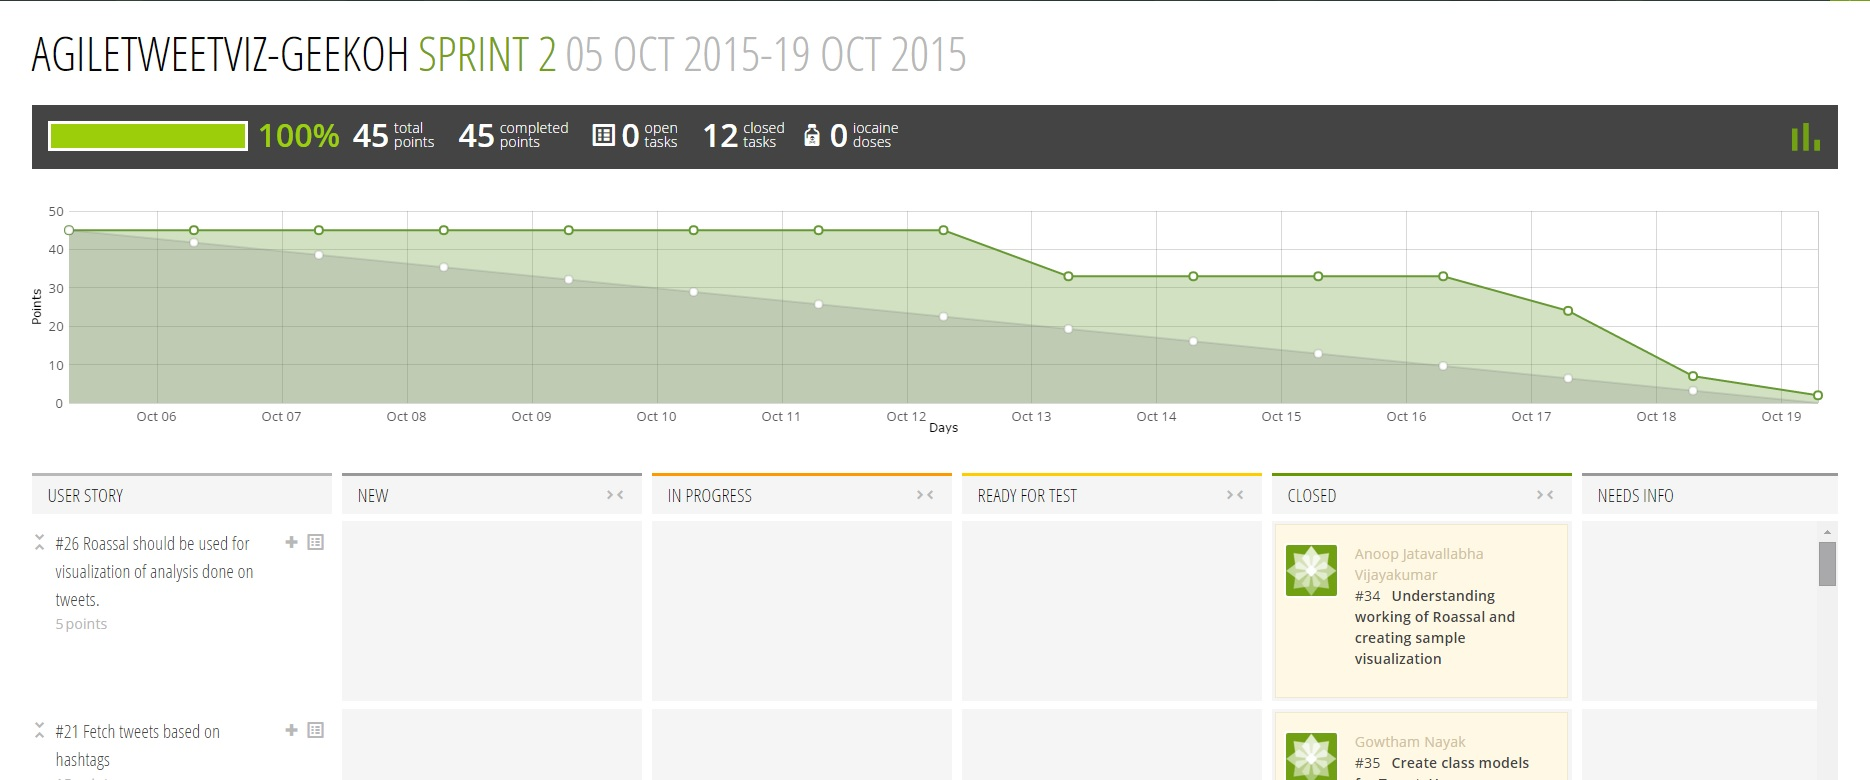
\includegraphics[width=6cm, height=6cm]{SprintBoard.jpg}
\caption{Virtual Sprint Board in Taiga}
\end{figure}

Each user story was provided with unique ID for traceability and a point (5, 10, 15) based system for prioritization. Every user story or task was also provided with an acceptance test(figure 6).

For any task that did not involve coding, a knowledge base document was written to explain the final outcome of the task. For example, our first sprint mostly consisted of the tasks that involved learning new platforms like MOOSE, PHARO, etc. In this case, a document was prepared explaining the concepts learned and shared with the team. Issues were logged in the Taigas issue tracker tool. 

\begin{figure}[!ht]
\centering
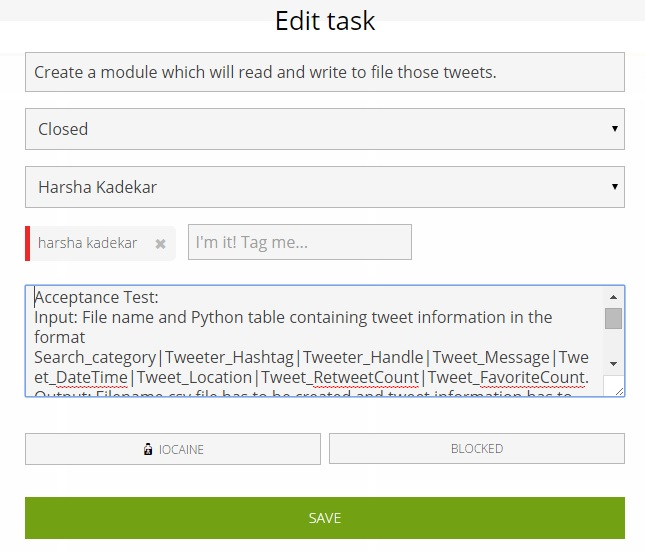
\includegraphics[width=6cm, height=6cm]{TaskInfo.jpg}
\caption{Task information in Taiga }
\end{figure}

Google site was a bird eye view of what was going on in the team. Every sprint and stand-up meeting details were recorded, including time of the meeting and important points discussed. Documents related to the process and product were placed in the wiki section of the site. Google Site proved to be a great tool for tracking the progress of the project and the artifacts being produced by the team.

There were two scheduled reviews for Quality Assurance. These reviews were performed by Dr. Kevin Gary after sprint 2 and sprint 5. The feedback after first review were: 1) User stories are not formed correctly - This should be the place holder for the conversation with the customer. 2) Many of the tasks were being closed  nearing the end of the sprint. Both of these points were taken into account and further improved on.

\section{Implementation}
As mentioned in the architecture, there are three main modules in this product. Tweet Fetch, Tweet Analysis and Tweet Visualization. 

Tweet Fetch module was completely developed using python. Various packages used for implementation are:
\begin{itemize}
\item Tweepy - Fetch tweets from Twitter.
\item Mysql Connector - Interact with MySQL database.
\item NLTK - For natural language processing of user input.
\item Py2Exe - To convert the python scripts to a deliverable.
\end{itemize}

Best coding practices including naming conventions for variables, functions, files and folders, comments and logging were discussed and followed throughout the project. All the commits to the Git were accompanied by the taskid and a brief explanation of the changes made to the code.

\begin{figure}[h]
\centering
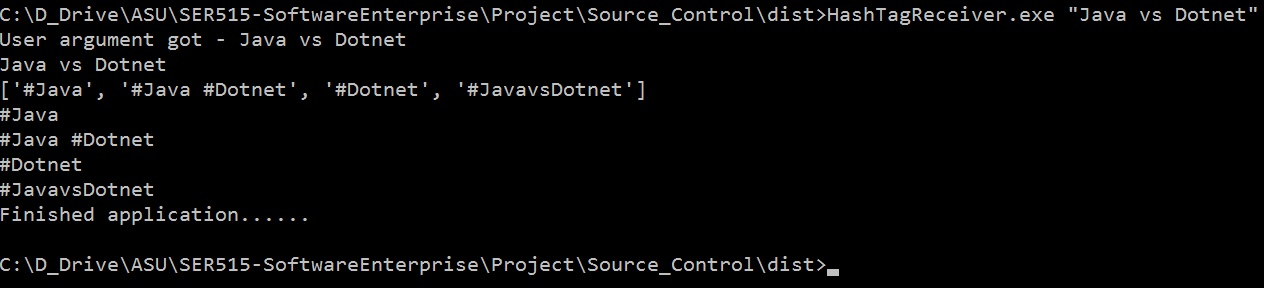
\includegraphics[width=\textwidth]{TweetFetchImp.jpg}
\caption{Tweet Fetch module execution}
\end{figure}

Tweet Analysis and Tweet Fetch modules were developed in SmallTalk based Pharo platform. Pharo and MOOSE has inbuilt source control. All the packages created in the "package-cache" folder of MOOSE were also checked into Git with proper comments.

Visualizations developed during the course of our implementation

\begin{enumerate}
\item Given a set of tweets based on a search category, we are able to get the hashtag's relationship. Initial aqua color ellipse in the figure 8, is user input whereas purple ellipses are the hashtags generated from the user input and red color boxes represent the next level of hashtags.
\begin{figure}[h]
\centering
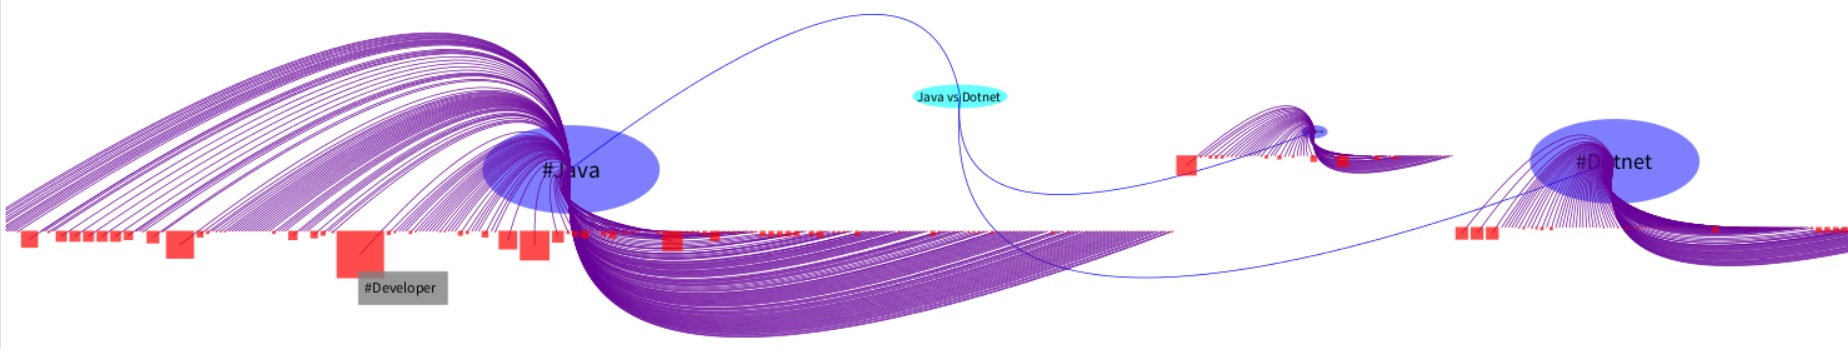
\includegraphics[width=\textwidth, height=2cm]{JustHashTags.jpg}
\caption{Hashtag relationship}
\end{figure}
\item Once the hashtag's relationship has been generated, the tweets were added in the visualization. In figure 9, green color ellipses in the outer circumference represents the tweets. Blue color ellipse is the main hashtag whereas red color boxes are sub hashtags. Size of the red color boxes depends on the number of tweets associated with that hashtag.

\begin{figure}[h]
\centering
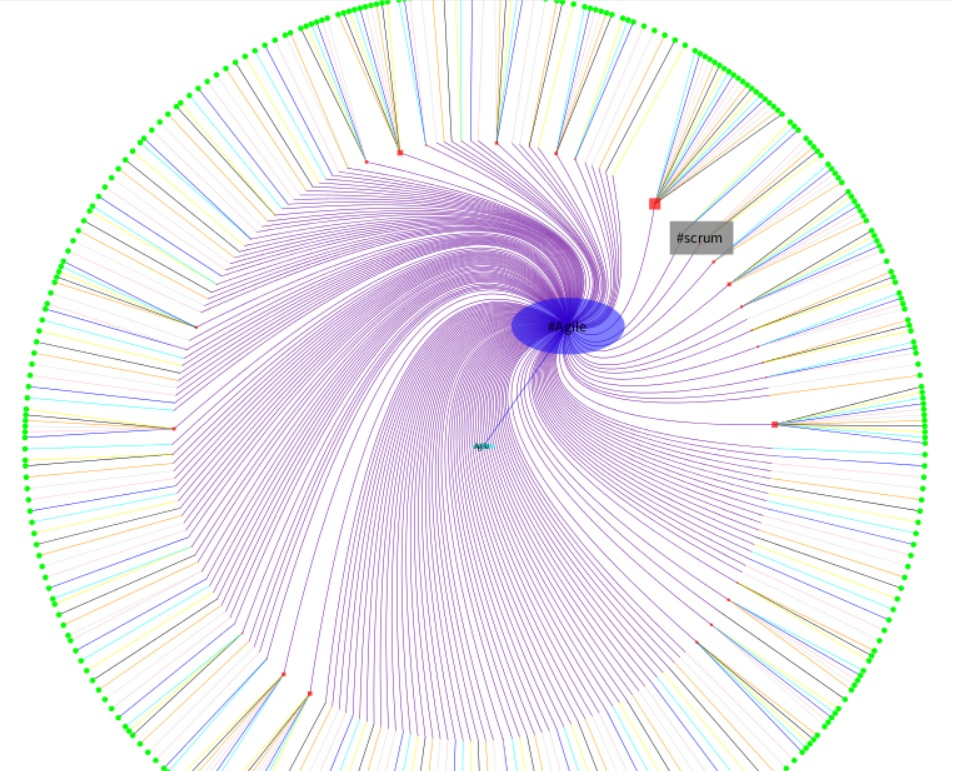
\includegraphics[width=5cm, height=5cm]{HashtagToTweets.jpg}
\caption{Tweet - hashtag relation}
\end{figure}

\item In figure 10, we have generated visualization based on users and their tweets. Here purple ellipses are users and red color boxes are tweets. Size of ellipse is dependent on the number of tweets by that user. Initially, users and tweets are displayed separately. Once the "connect" Button clicked(figure 11), all the tweets tweeted by a user will come together and circle around that user.
\begin{figure}
\centering
\begin{minipage}{.5\textwidth}
\centering
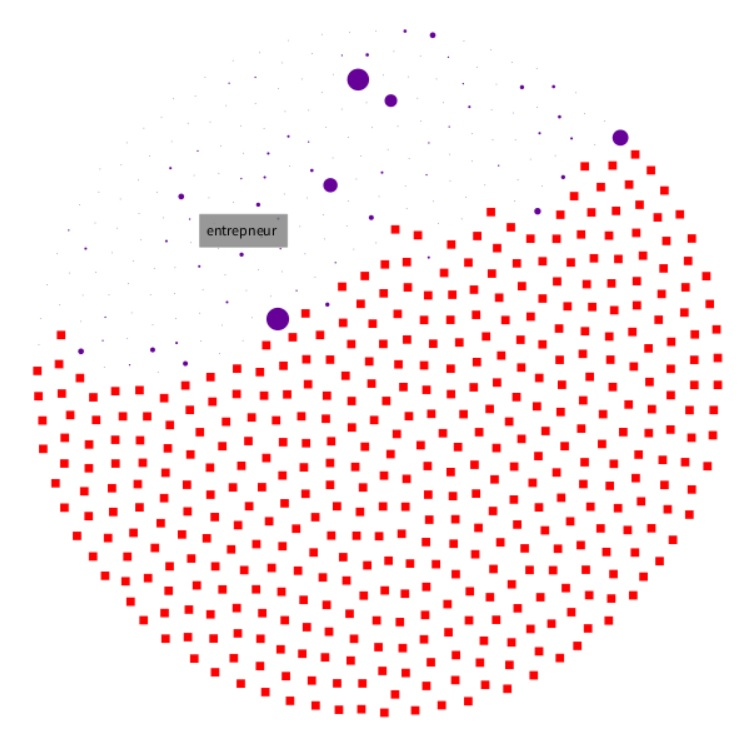
\includegraphics[width=.6\linewidth]{UserTweet1.jpg}
  \caption{User and tweets}
\end{minipage}%
\begin{minipage}{.5\textwidth}
\centering
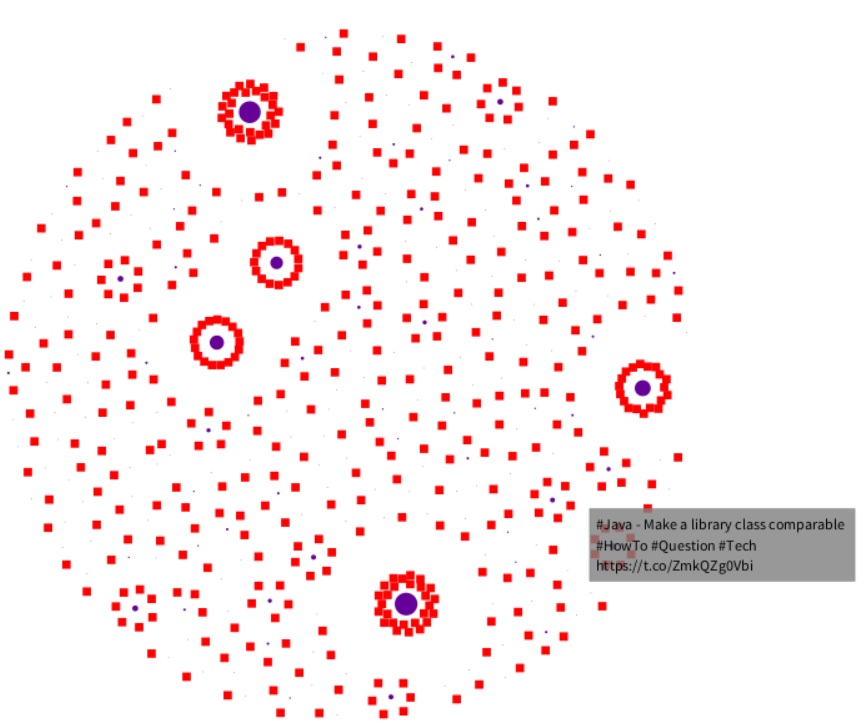
\includegraphics[width=.6\linewidth]{UserTweet2.jpg}
  \caption{Connected User and tweets}
\end{minipage}
\end{figure}

\item Popularity of a hashtag in terms of simple graphs(Figure 12).
\begin{figure}[h]
\centering
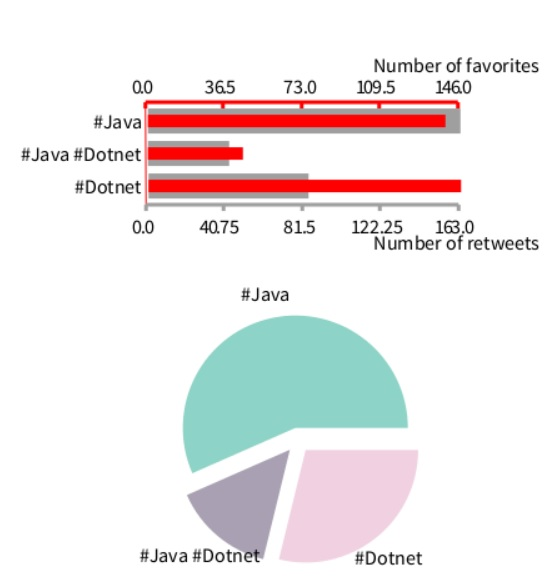
\includegraphics[width=6cm, height=6cm]{Graph.jpg}
\caption{Popularity of tweets}
\end{figure}


\end{enumerate}

\section{Validation and Verification}
Taiga was the tool used to report and track any issues during the time of product development.

\begin{figure}[h]
\centering
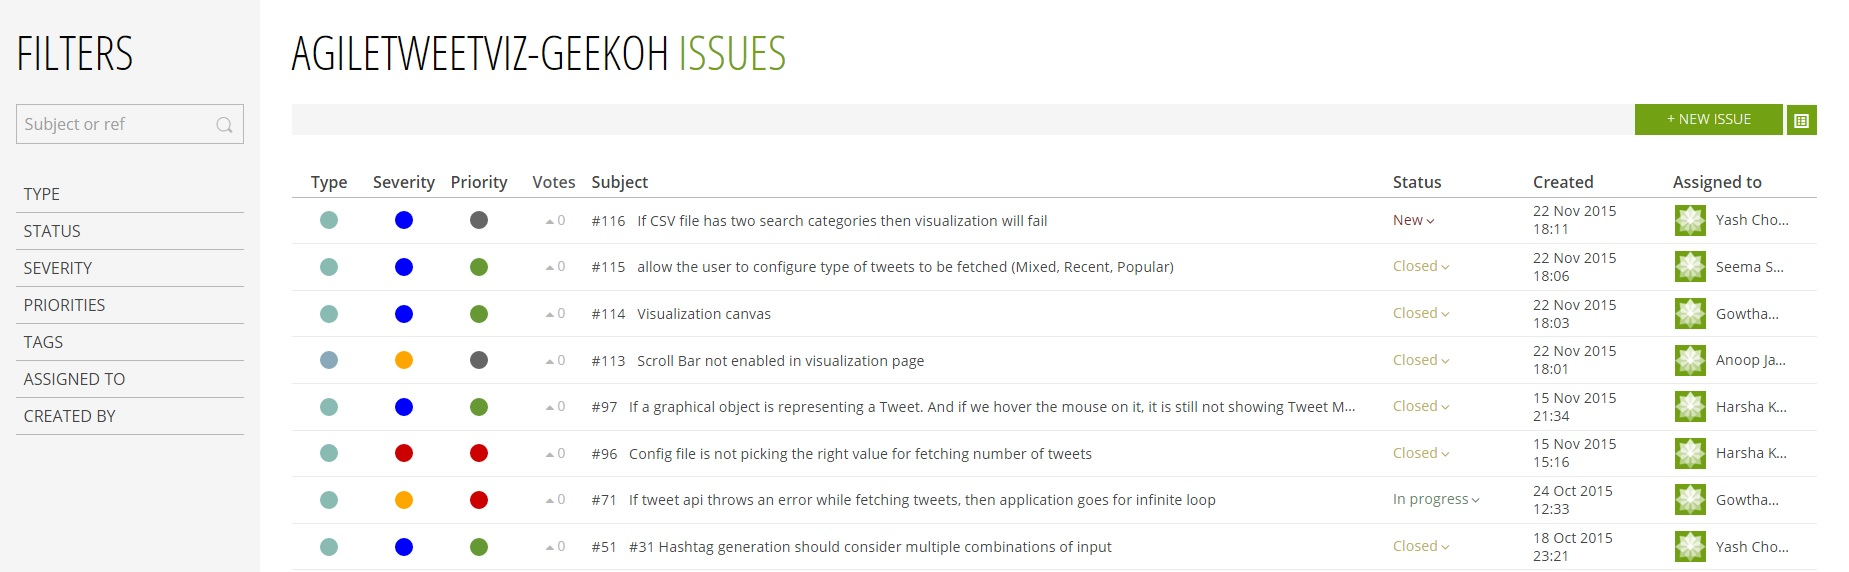
\includegraphics[width=\textwidth]{Issues.jpg}
\caption{Issues list in Taiga}
\end{figure}

Every issue when being logged, has to mention the task under which this issue has occurred unless it was discovered during regression or system integration testing. Taiga gives the classification of issues as bug, question or enhancement. Apart from that, priority is provided as low, medium or high. It also classifies the bugs as severity:  minor, normal, important, critical or wish-list. Any issue can be in one of the stages: New, In-progress, Ready for test, Closed, Needs Info, Rejected, Postponed. 

\begin{figure}[h]
\centering
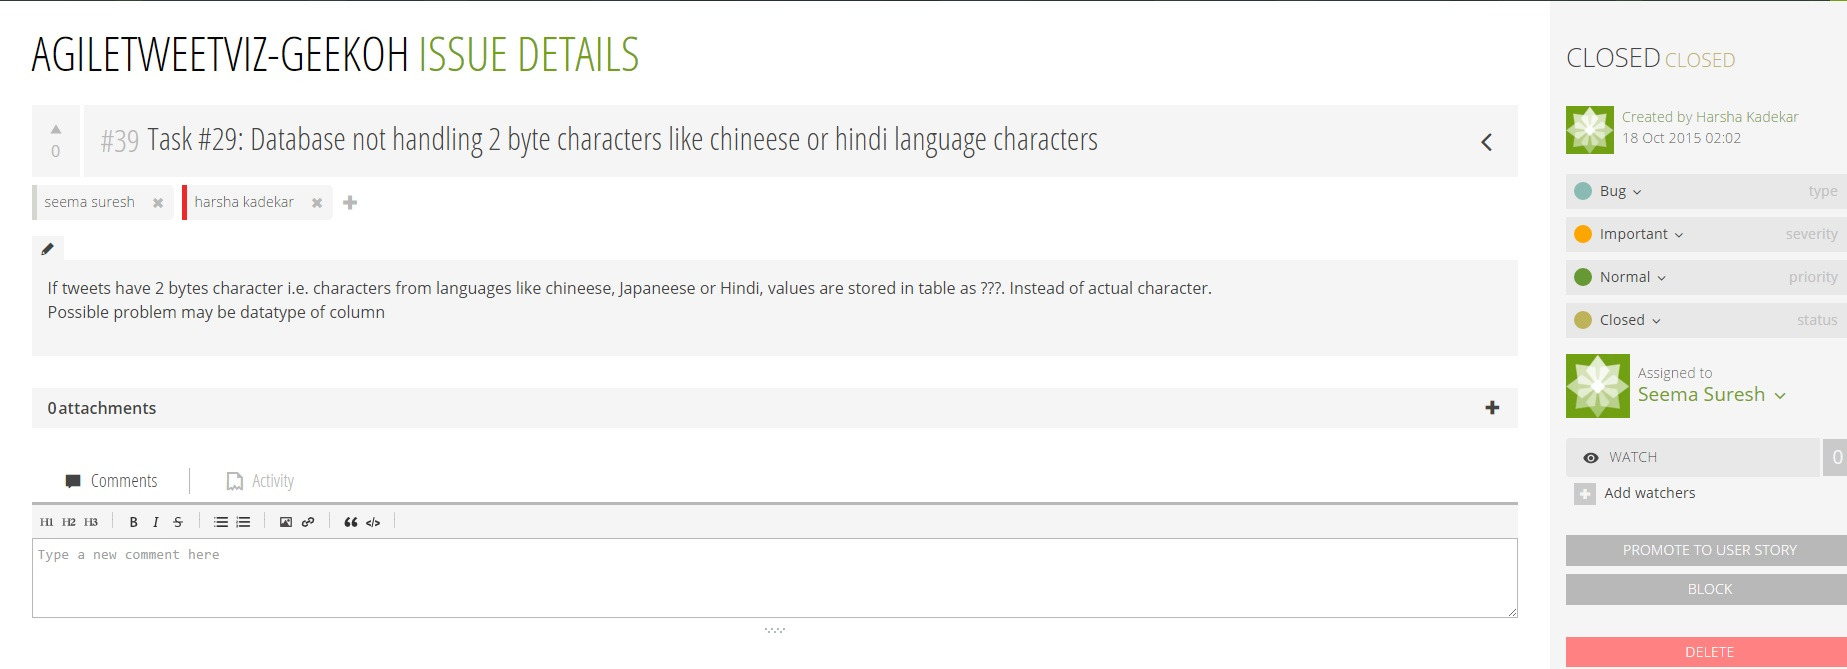
\includegraphics[width=\textwidth]{Issue2.jpg}
\caption{Issue tracking in Taiga}
\end{figure}

Three Amigos rule was followed while moving the task from In-Progress to Complete state, where three Amigos included developer, tester and requirement owner.


Apart from the acceptance test, we also had Integration test cases and Regression test cases. Sprint 5 was dedicated for the integration and regression testing. 

Based on the discussion with product owner, Hapao will be used as test coverage tool in the future.

\section{Outcomes and lessons learned}
After every sprint we conducted Retrospectives to judge and reflect on our progress so far. Some of the highlighted points of the project are mentioned below divided in the categories as they were discussed: -

\textbf{What worked well for us?} 
\begin{itemize}
\item Agile process
\item Pharo/ Roassal
\item NTLK and Tweepy library
\item Changing vision of Project
\item Even work distribution
\end{itemize}

Our biggest accomplishment in this project was learning of the new tool - Pharo/Roassal and successfully implementing agile process for software development. As a team, we enjoyed working in Agile environment as it helped us distribute work evenly among team members and throughout the project. Also considering that a new tool had to be learned and implemented for this project, agile did not force us to master Pharo beforehand. In fact, we learned the tool as and when demanded by sprints and user stories. Agile was also helpful in accommodating our code with evolving requirements as updated by our sponsor thus providing us with the ability to start contributing to product development from the beginning. To accept hashtag and download tweets, we used pythons built in library that helped to automate the initial process, thus giving us enough time to learn and explore Roassal. Slowly as we learned Roassal better, this led to evolving vision of our project, which in turn was very well accommodated by Agile process.

\textbf{What did not work well for us?} 

\begin{itemize}
\item Could not exploit all the features of Roassal
\item Unequal commitment of team members
\item Changing vision of Project
\end{itemize}

Since Pharo/Rossal is a very new development tool, finding an online community was difficult. It made the learning process harder and thus more time was spent on learning the tool rather than testing its limits to achieve better visualizations. We used the examples mentioned in Roassal library for better understanding and went beyond the examples to create new and vivid visualizations. This process led to several visualizations which were not necessarily required but, it helped us understand the tool better and clarify our vision for the project. Lack of clear understanding of initial requirements lead to some extra coding work that could have been avoided. For example, we focused on User Interface for the initial sprints but later it was determined that it was not required. Similarly, in the first few sprints more importance was given to learning of tools, which resulted in development of features which were not aligned to vision of the product.

\textbf{What actions can we take to improve our process going forward?} 

\begin{itemize}
\item Better implementation of Agile process 
\item Automate unit tests
\item Improve the task break down of an User Story
\item Division of tasks among team members with in each user story rather than dividing complete user story among team members.
\item Review the changes to vision in each sprint.
\end{itemize}

There was always room for us to improve on Agile process. For example, contrary to agile method we were more comfortable in assigning one user story to one team member rather than assigning individual tasks of user story to individual member and moving stories at constant pace. We were also unable to implement efficient daily stand-up meetings due to the schedule problems. We followed a Test Driven Development process where we spent a lot of time in checking our code manually after making any change. Automation of tests could not be implemented due to lack of time. 

\section{Future Work, Acknowledgment and Conclusion}

We believe this is just the beginning of the project, there is still a lot of scope for improvement. Some of the important tasks which we are working on are :
\begin{enumerate}
\item Map the users through the hashtags used. Categorize the users into different groups based on the hashtag's popularity
\item Develop a single web interface for the whole product. User will provide input in a webpage. The input will be passed to our product in backend to process and generate the visualization. Once the visualization is done, it will be exported to HTML5 and shown to the user in the same webpage where input was given.
\item Currently product deliverables are present in the windows format. We are in the process of porting it to Linux/Unix and Mac environments.
\item Once we are able to categorize the tweets and the users based on our hashtag relationship, we would like to compare with the group categorization done via other methods as mentioned in the paper by \textit{Abhishek Sharma, Yuan Tian and David Lo}\cite{sehotintwitter} .
\end{enumerate}

For our project so far we have extracted more than 80,000 tweets in real-time using python and then analyzed them using our metamodel in Pharo. We have further created 6 visualization patterns using Roassal library, which reflects various relationships between tweets, users and hashtags. There are many improvements and visualizations that can be achieved via Pharo and Roassal respectively. For example, we would like to explore the emotional aspects in a tweet.

This project was a great experience as it introduced us to new technology, while giving a practical hands-on experience in agile work environment. We would like to thank our Professor, Dr. Kevin Gary, Arizona State University, for teaching and guiding us in the right path throughout the duration of project and helping us on Agile development process. We would also like to thank our sponsor Dr. Alexandre Bergel ,University of Chile, for giving us opportunity to work in Pharo/Roassal and guiding us from time to time about these technologies as well as helping us to understand the requirements.
\newpage
\begin{thebibliography}{7}
\bibitem{sehotintwitter}
Abhishek Sharma, Yuan Tian and David Lo.
\textit{What's Hot in Software Engineering Twitter Space?}.
2015 IEEE International Conference on Software Maintenance and Evolution (ICSME), 2015
\bibitem{AgileVisualization}
\textit{Agile Visualization Book}
\texttt{http://agilevisualization.com/\#book}
\bibitem{pharobyexample}
Andrew P Black, Stéphane Ducasse, Oscar Nierstrasz, Damien Pollet, Damien Cassou, Marcus Denker, Damien Cassou and Kilon Alios
\textit{Pharo by Example}
\texttt{http://pharobyexample.org/}
\bibitem{Deepintopharo}
Alexandre Bergel, Damien Cassou, Stéphane Ducasse and Jannik Laval
\textit{Deep into Pharo}
\texttt{http://www.deepintopharo.com/}
\bibitem{pharoinnutshell}
\textit{Pharo in a Nutshell}
\bibitem{roassalvisualization}
\textit{Agile Visualization with Roassal}
\texttt{http://pharobooks.gforge.inria.fr/PharoByExampleTwo-Eng/latest/Roassal.pdf}
\bibitem{MooseBook}
Tudor Girba
\texttt{http://www.themoosebook.org/book}
\bibitem{SoftwareEngineeringbook}
Ian Sommerville
\textit{Software Engineering, 10th Edition}
\texttt{http://iansommerville.com/software-engineering-book/}
\textit{The MOOSE book}
\bibitem{SCOREwebsite}
SCORE Agile Tweet Viz website
\texttt{http://score-contest.org/2016/projects/tweetviz.php}
\end{thebibliography}

\end{document}